\documentclass[11pt,a4paper]{article}
\usepackage[margin=23mm,top=23mm,bottom=22mm,headheight=15pt]{geometry}
\usepackage{fontspec}
\setmainfont{texgyrepagella}[Extension=.otf,UprightFont=*-regular,BoldFont=*-bold,ItalicFont=*-italic,BoldItalicFont=*-bolditalic]
\setsansfont{texgyreheros}[Extension=.otf,UprightFont=*-regular,BoldFont=*-bold,ItalicFont=*-italic,BoldItalicFont=*-bolditalic]
\usepackage{unicode-math}\setmathfont{texgyrepagella-math.otf}
\usepackage{graphicx,booktabs,tabularx,longtable,array,amsmath,amsthm}
\usepackage{xcolor,enumitem,microtype,fancyhdr,caption,float,titlesec,xurl}
\usepackage[hidelinks,unicode]{hyperref}
\definecolor{ink}{HTML}{304750}\definecolor{sage}{HTML}{687C69}\definecolor{copper}{HTML}{AF6843}\definecolor{paper}{HTML}{F4F2EC}
\titleformat{\section}{\Large\bfseries\color{ink}}{}{0pt}{}
\titleformat{\subsection}{\large\bfseries\color{ink}}{}{0pt}{}
\setlength{\parindent}{0pt}\setlength{\parskip}{6pt plus 1pt minus 1pt}
\setlength{\emergencystretch}{3em}\linespread{1.07}
\setlist{nosep,leftmargin=1.4em}
\captionsetup{font=small,labelfont={bf,color=ink},justification=raggedright,singlelinecheck=false,skip=6pt}
\pagestyle{fancy}\fancyhf{}\fancyhead[L]{\small\sffamily\color{ink}Checkers with Runway 13}\fancyhead[R]{\small\sffamily\color{sage}RESEARCH WHITE PAPER · V3}\fancyfoot[C]{\small\thepage}\renewcommand{\headrulewidth}{.3pt}
\newcommand{\parthead}[2]{\section{\texorpdfstring{\textcolor{copper}{\small\sffamily PART #1}\quad #2}{Part #1 — #2}}}
\newcommand{\fig}[4]{\begin{figure}[H]\centering\includegraphics[width=#2\textwidth]{figures/#1.pdf}\caption{#3}\label{#4}\end{figure}}
\newcommand{\insight}[2]{\par\smallskip\noindent\textcolor{copper}{\textbf{#1}}\quad #2\par\smallskip}
\newcommand{\R}{\mathbb R}\newtheorem{proposition}{Proposition}
\hypersetup{pdftitle={Checkers with Runway 13},pdfauthor={Aryan Ayyar},pdfsubject={Research white paper, Version 3; mathematical and historical investigation of Kai Tak}}
\begin{document}\raggedbottom
\hypersetup{pageanchor=false}
\begin{titlepage}\thispagestyle{empty}
{\sffamily\small\color{sage}INDEPENDENT RESEARCH WHITE PAPER\hfill VERSION 3 · 13 OCTOBER 2026\par}
\vspace{14mm}
{\fontsize{37}{42}\selectfont\bfseries\color{ink}Checkers with\\Runway 13\par}
\vspace{6mm}{\large Aryan Ayyar\par}
\vspace{8mm}
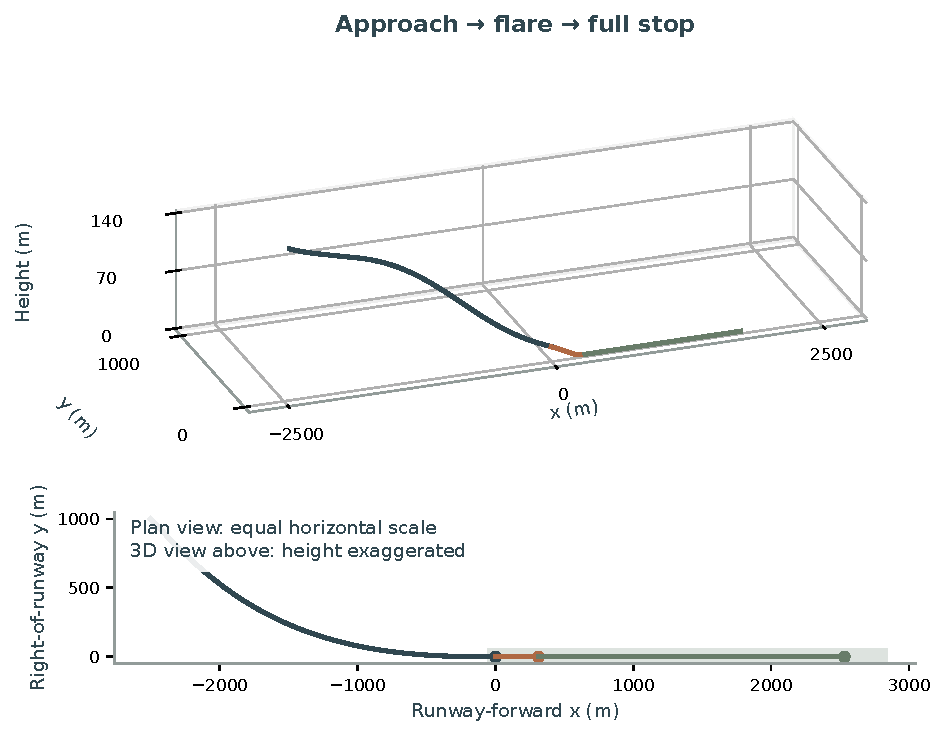
\includegraphics[width=\textwidth,height=110mm,keepaspectratio]{figures/09_complete_calm.pdf}\par
\vspace{5mm}
{\Large\color{ink}How could a 747 turn over Kowloon,\\find the runway, and still have room to stop?\par}
\vspace{5mm}
A historical investigation and an explicit mathematical landing, with the boundary between the two kept visible.
\vfill
{\small Cover: the project's calm-air mathematical reference, not a recovered historical flight. Editable sources, figure inputs and verification accompany this edition. Independent working white paper; not peer reviewed or operational flight guidance. The author's foreword is marked for review.\par}
\end{titlepage}
\hypersetup{pageanchor=true}\setcounter{page}{2}
\section*{Author's foreword}
{\small\sffamily\color{copper}FIRST-PERSON DRAFT FOR ARYAN AYYAR'S REVIEW}\par\medskip
Long before I had a research question, I had an image: a large aircraft turning above Hong Kong, close enough to the city for the buildings to seem part of the approach. I was fascinated by aircraft as a child, particularly by the engineering that allowed something so large to move with such apparent precision. Kai Tak gave that fascination a setting. The Checkerboard approach looked like a problem that should not have had enough room for its solution.

Watching Richard Hammond's \emph{Engineering Connections} encouraged a particular way of looking at such things. The spectacle was an invitation to ask how the pieces worked together. A remarkable structure or machine became more interesting when its mechanisms were explained. I wanted the same explanation for Kai Tak. How much of the turn came from the aircraft's capabilities, how much from the shape of the approach, and how much depended on the person flying it?

The imagery and music of \emph{Enter the Dragon} belong to that early fascination too. In my memory, aircraft and historical Hong Kong became associated with a city whose geography seemed unusually present in its everyday life. That association is personal, not documentary evidence about a particular flight or filming location. It helped make the question memorable; it could not answer it.

Years later, while studying for a Master of Finance at Hong Kong Polytechnic University and living in Tsim Sha Tsui, I became more attentive to the city's geography and engineering history. The harbour, the hills and the density of the built environment made the old airport feel less like an isolated aviation curiosity. It was part of a larger question about how Hong Kong made demanding arrangements work. My own time in the city came after Kai Tak had closed. Arriving at the modern airport at Chek Lap Kok was not experiencing the former Runway 13 approach.

I returned to the question with tools developed through research in financial economics and mathematics. I am not a trained aerospace engineer. That matters: an equation I can solve is not automatically an adequate account of an aircraft, and a convincing reconstruction is not automatically a survey. The attraction of the project lies partly in discovering where the mathematics is useful and where it must wait for better evidence.

This paper follows that process. It begins with the airport and moves towards a complete mathematical landing, including the less photogenic business of stopping. Along the way, it asks what can be recovered from dated photographs, maps and published flight records, and what those sources leave unresolved. I hope it preserves something of the original curiosity without using wonder as an excuse for imprecision. The approach becomes more impressive, not less, when we can explain some of its demands and say honestly which questions we have not yet answered.

\vfill{\small This foreword records the author's supplied motivation. It is not a historical source or a claim of professional aerospace qualification.}
\clearpage

\section*{The investigation in brief}
Kai Tak's Runway 13 approach joined an instrument-guided descent to a visual right turn over Kowloon. The celebrated $47^\circ$ was a change between published magnetic directions, not the aircraft's bank angle. The engineering problem was to coordinate geometry, speed, descent, visual acquisition and stopping distance within a crowded landscape.

This paper makes that coupling inspectable. A reduced aircraft model constructs an explicit approach, flare, touchdown and full stop. Two retained scenarios have separate computer-assisted continuous-time feasibility certificates. Dated maps, aerial photogrammetry and CAL605 recorder and weather evidence show what would be required to connect those mathematical paths to historical reality.

\begin{table}[H]\centering\small
\caption{Verified model outcomes. Identical illustrative braking: 2 s delay, then $0.15g$. Synthetic entry and corridor; no historical obstacle-clearance claim.}
\begin{tabular}{@{}lrr@{}}\toprule
 & Calm-air witness & Steady-wind witness\\\midrule
Touchdown beyond threshold & 313.49 m & 302.11 m\\
Full-stop station & 2,531.32 m & 2,233.23 m\\
Runway remaining (LDA 2,786 m) & 254.68 m & 552.77 m\\
Certified normalized margin, at least & 0.0397 & 0.15079347\\
Necessary family upper bound & $<0.1559772$ & $\leq0.21674438$\\\bottomrule
\end{tabular}
\end{table}

The wind case imposes a uniform, steady wind from $070^\circ$ true at 21 knots. Its additional 298.09 m of remaining runway is a difference between separately optimized scenarios, not an identified causal wind effect or a demonstrated improvement over a historical procedure. Neither optimum is located by the available bounds.

\subsection*{A route through the paper}
\begin{tabularx}{\textwidth}{@{}rXr@{}}
I & The airport that challenged intuition & p.\,\pageref{part:1}\\
II & Reconstructing a lost airport & p.\,\pageref{part:2}\\
III & The mathematics of the impossible-looking turn & p.\,\pageref{part:3}\\
IV & Can we construct a complete landing? & p.\,\pageref{part:4}\\
V & What happens when wind changes? & p.\,\pageref{part:5}\\
VI & What did the historical evidence reveal? & p.\,\pageref{part:6}\\
VII & What we have proved, and what remains unknown & p.\,\pageref{part:7}\\
VIII & A public research resource for Hong Kong & p.\,\pageref{part:8}\\
 & Mathematical derivations and reproduction & p.\,\pageref{app:dynamics}\\
\end{tabularx}

\medskip\textbf{The central distinction.} A mathematical certificate verifies a trajectory against declared equations and constraints. An aviation-safety finding requires validated aircraft behaviour, complete relevant obstacles, operational procedures and uncertainty evidence. The current work supplies the former in restricted scenarios, not the latter.
\clearpage

\parthead{I}{The airport that challenged intuition}\label{part:1}
From the ground, a large aircraft turning above a city looks like a contest between scale and space. At Kai Tak the setting made that impression unusually vivid: built-up Kowloon on the approach side, rising terrain beyond, and a runway extending into Kowloon Bay. The airport was not simply a long strip of pavement. Its usefulness depended on how aircraft could reach it.

\fig{01_historical_airport}{.79}{The airport and its immediate urban setting in Lands Department frame A36143. The annotations identify visible features; no flight track is overlaid. Catalogue date: 2 November 1993; the handwritten frame label appears to read 3 November, an unresolved source-date discrepancy. Original scan orientation, not north-up; no metric scale is inferred from this perspective photograph. Source: Lands Department, HKSAR Government; CSDI Portal and DATA.GOV.HK, open-data DAP-L0. Intellectual-property ownership retained by the Government; supplied as-is, without endorsement.}{fig:airport}

A runway-aligned instrument approach would have pointed aircraft towards a different surrounding landscape. Runway 13 instead used an offset Instrument Guidance System (IGS), followed by visual manoeuvring. The Civil Aviation Department dates the IGS introduction to 1974; it improved runway use in adverse weather but did not remove the final visual requirement \cite{cadhistory,cad}.

The question is not whether a 747 can turn. It plainly can. The question is whether the turn can finish at the right place, height, speed and orientation, with enough runway left for the rest of the landing.
\clearpage
\subsection*{What the Checkerboard approach actually asked of a pilot}
The IGS supplied lateral guidance along a localiser and vertical guidance on a $3.1^\circ$ glidepath. In the 1993 report, its localiser centreline is $088^\circ$ magnetic; the runway direction is $135^\circ$ magnetic. Both bearings use the same reference, so their difference is $47^\circ$. That is an angular change in direction on a plan, not a command to bank the wings by 47 degrees.

\fig{02_approach_geometry}{1}{Published directions and the instrument-to-visual sequence. Bearings are clockwise from magnetic north. The rays share an origin only to compare angles: their meeting point is not a surveyed turn location, and the diagram is not a navigational chart. Source: CAD Report 1/95, sections 1.8.1 and 1.10, Appendix 1. Ground track and air heading differ in wind.}{fig:geometry}

The instrument segment ended at the middle marker, reported as 1.7 nautical miles from touchdown. If visual flight had not been achieved there, the report specifies a missed approach \cite[§1.8.1]{cad}. The famous final turn therefore was not something the IGS could guide to completion in zero visibility. Checkerboard Hill was a visual reference in Kowloon, not a landmark on Victoria Peak across the harbour. The CAD's retrospective account describes the visual right turn over Kowloon City \cite{cadlink}.

The approach distributed different jobs among navigation equipment, a published procedure, visual references and the crew. Terrain and buildings shaped the available geometry. Wind altered the relation between where the nose pointed and where the aircraft travelled. A successful alignment still had to deliver an acceptable touchdown.

The 1993 case report gives 3,331.5 m of runway length, 61 m width and 2,786 m of landing distance available (LDA) \cite[§1.10]{cad}. The last number governs the threshold-relative stopping calculation here. A general airport history lists a 3,390 m extension-era length \cite{cadhistory}; these source quantities are not silently substituted for one another. Likewise, the airport that closed in July 1998 must not be confused with the replacement at Chek Lap Kok \cite{cadlink}.

\insight{The mathematical question}{Can one continuous motion satisfy the demands of turning, descent, alignment, touchdown and stopping together? A solution must fit all of them, not merely look plausible from one viewpoint.}
\clearpage

\parthead{II}{Reconstructing a lost airport}\label{part:2}
A modern satellite image answers a modern question. For a landing in 1993, a building erected later is an anachronism; a demolished building missing from today's database may be the very obstacle that mattered. Reconstructing Kai Tak starts by attaching dates and coordinate meanings to evidence, before constructing a city from it \cite{maps,photos}.

\fig{03_dated_maps}{1}{Two editions of survey sheet 11-NE-11A, October 1989 and July 1994, in the same Hong Kong 1980 Grid rectangle. North is up; axes are metre offsets and the bar is 100 m. Numbered labels locate named map forms, not accepted unchanged 1993 buildings. Registered raster spacing is 0.25 m, not measured positional accuracy. Source: Lands Department, HKSAR Government; CSDI Portal and DATA.GOV.HK, Old Survey Sheets. Government intellectual-property ownership retained; supplied as-is, without endorsement.}{fig:maps}

The project acquired 227 valid survey-map archives across 93 core sheet locations and 48 full aerial frames. These are substantial source holdings, but counts do not measure coverage of every obstacle. Map editions may carry forward old information. A photograph observes visible surfaces at one moment; it does not show what lies behind a roof or inside an occlusion.

The paired maps make change inspectable. Four road-cell comparisons contain 404 dated assignments of 202 current templates, alongside 531 dated map-region assignments and 397 cross-date overlaps. These are matching candidates, not 935 verified historical buildings. A geometrical overlap cannot establish that a building retained its height or identity between editions.

Documentary building chronology is a third source, useful for testing proposed identities and presence dates. It does not turn a current footprint into a historical roof. This distinction matters especially for structures removed or altered around the selected period.

\textbf{Working epoch.} The landing case is 4 November 1993. The stereo pair uses the catalogue's 2 November date; the A36143 scan-label discrepancy in Figure~\ref{fig:airport} remains unresolved. Neither date resolves all intervening changes or authenticates a complete city model.
\clearpage
\subsection*{What two photographs can recover}
Stereo reconstruction uses displacement between corresponding image features to infer relative three-dimensional structure. The camera geometry and metric scale must also be determined. Here, frames A36142 and A36143 provide overlapping views; image matches are anchored to manually interpreted ground features and survey-road controls. Camera and scan assumptions remain part of the reconstruction.

\fig{04_reconstruction}{1}{Historical stereo reconstruction, shown as every fifth retained point. Left: grey points extend beyond the map-control hull; copper points lie inside it. Right: conditional surface elevation above a fitted local park/road plane, with colour clipped outside the indicated range. Neither vertical coordinate is HKPD or height above each building's own ground. Diagnostic HK1980 positions; gaps remain gaps. Derived from Lands Department A36142/A36143 open-data photographs and survey controls; Government/CSDI/DATA.GOV.HK attribution and ownership retained.}{fig:reconstruction}

The settled reconstruction retains 1,318 sparse matches and 171,307 filtered dense points; 3,780 dense points lie inside the map-control hull, about 2.21\%. The distinction is easily missed in a convincing rendering. Many points can be reconstructed outside the small region in which control geometry directly supports the alignment. A held-out horizontal control discrepancy of 5.754 m RMS is a diagnostic of that fit, not a vertical roof-error guarantee.

A conservative mesh connects 155,891 vertices into 225,371 triangles. Its 86,061 boundary edges reflect an open, non-watertight surface. Connecting points does not discover hidden building walls or fill an occlusion with evidence. The retained geometry includes a prior 49-point interpolation-support correction; the invalidated predecessor is not used.

\insight{Insight 1: a dense image can contain sparse knowledge}{The fraction $3780/171307\approx0.0221$ measures local control support, not the fraction of the city proved accurate. More triangles can improve visual continuity without improving surveyed clearance. This is a property of the evidence, not a verdict against photogrammetry.}
\clearpage
\subsection*{The latest obstacle evidence: useful, still incomplete}
Version 3 adds the repository's settled obstacle handoff. It contains 24 approximate mapped surface-elevation readings at 12 sites on sheet 11-NW-10D, from the November 1989 and June 1995 editions. The printed legends identify metre elevations above Hong Kong Principal Datum (HKPD) and describe the spot readings as approximate. Repeated values may be carried-forward cartography, not independent surveys.

\begin{table}[H]\small
\caption{Different geometric evidence answers different questions. Source: settled reconstruction and obstacle reports; modern product documentation \cite{dtm,buildings}.}
\begin{tabularx}{\textwidth}{@{}p{.24\textwidth}p{.24\textwidth}X@{}}\toprule
Evidence & What is available & What does not follow\\\midrule
Dated map faces & 45 reviewed dated forms for 15 named forms & Not 45 distinct buildings; historical tops remain unknown.\\
Mapped spot elevations & 24 readings at 12 sites & No bound on intervening terrain, roofs, antennas or vegetation.\\
Stereo points & Relative-plane surfaces & No absolute vertical datum or complete obstacle volume.\\
Modern 5 m DTM & 2014--2015 source photography; 2019 revision & Not a 1993 terrain/obstacle census; product accuracy is not a worst-case bound.\\
Modern buildings & September 2026 snapshot & Historical presence and unchanged height cannot be inferred.\\\bottomrule
\end{tabularx}\end{table}

A roof elevation above HKPD is not a building height to add to a terrain elevation. Both may already use the same vertical origin. Conversely, the accident report's runway elevation of 15 ft AMSL, or 4.572 m in its stated reference, cannot be reconciled with HKPD merely by assuming that all notions of ``sea level'' coincide. The project has not accepted that transformation.

The latest inventory therefore records zero complete obstacle volumes, zero physical obstacle upper bounds, and \texttt{historical\_clearance\_ready=false}. These are explicit scientific outcomes. An unknown-coverage polygon remains in the exported geometry so that an unmeasured region cannot quietly become empty airspace.

Even perfect building heights would not complete the clearance problem. A point-mass trajectory has no wingspan, tail or landing gear. A real aircraft sweeps a volume through space, and its actual path differs from the reference. To certify clearance, that volume and a justified tracking allowance must avoid appropriately bounded historical obstacles along the whole motion.

The reconstruction is already valuable as an inspectable historical resource. Its present contribution is to locate evidence, expose dating and datum problems, and make future corrections possible. It is not yet an input capable of certifying the two landing scenarios that follow.
\clearpage

\parthead{III}{The mathematics of the impossible-looking turn}\label{part:3}
\subsection*{A large change of direction need not mean a large bank}
In a steady, coordinated, level turn in still air, lift $\mathcal L$ must support weight and provide centripetal acceleration. If $\phi$ is bank angle, $V$ airspeed and $R$ turn radius,
\begin{equation}
\mathcal L\cos\phi=mg,\qquad \mathcal L\sin\phi=\frac{mV^2}{R}
\quad\Longrightarrow\quad R=\frac{V^2}{g\tan\phi}.
\label{eq:turn}
\end{equation}
Mass cancels from this ideal geometric relation. It has not disappeared from the lift, stall, structural or thrust requirements of the aircraft.

\fig{05_turn_physics}{1}{Radius and time to change direction by $47^\circ$, computed from equation~\eqref{eq:turn}, $t=R\Delta\psi/V$, and $g=9.80665$ m/s$^2$. Speeds 70, 78 and 85 m/s are illustrative true airspeeds. Constant-speed, level, coordinated turns; instantaneous entry into bank is not modelled. These curves are explanatory benchmarks, not Kai Tak flight reconstructions.}{fig:turn}

At 78 m/s and $15^\circ$ bank, the ideal radius is 2,315 m. A $47^\circ$ change takes 24.35 s and 1,899 m of arc. The associated load factor is $1/\cos15^\circ=1.0353$. The example explains how a visually substantial direction change can accumulate under a moderate bank, provided enough space and time are available. It does not show that this particular arc fits the historical approach.

\insight{Insight 2: direction change is accumulated}{The wings need not bank by the desired final change of heading. Bank produces a turn rate, $\dot\psi=g\tan\phi/V$; integrating that rate produces the heading change. Roll-in and roll-out consume additional time and alter the geometry.}

The real research candidate allows speed, descent and bank to vary together. The simple formula is a way into that coupled problem, not a substitute for it.
\clearpage
\subsection*{The air and the ground do not agree on velocity}
An aircraft responds aerodynamically to its motion through air. A runway measures the aircraft's motion over the ground. For constant wind velocity $\mathbf w$,
\begin{equation}
\underbrace{\dot{\mathbf r}}_{\text{ground velocity}}
=\underbrace{V\mathbf e_V}_{\text{air velocity}}+\underbrace{\mathbf w}_{\text{wind velocity}}.
\label{eq:wind}
\end{equation}
The direction of $\dot{\mathbf r}$ is ground track; the horizontal direction of $\mathbf e_V$ is air heading. In a crosswind, maintaining a runway-aligned track can require a heading offset. A ground-track change of $47^\circ$ does not prescribe the same air-heading change in every wind.

\fig{06_wind_vectors}{1}{Left: horizontal velocity triangle at the wind candidate's touchdown. Forward/right axes are runway-relative; the right axis increases down the panel. Right: projection of the same steady wind onto changing track directions, from $-47^\circ$ to runway alignment. Source: frozen wind input and endpoint state. Wind is \emph{from} $070^\circ$ true at 21 kt; assumed runway bearing is $133^\circ10'$ true. The plot describes constant wind, not recovered gusts.}{fig:wind}

Using the chart convention $135^\circ$ magnetic minus $1^\circ50'$ west variation gives a true runway bearing of $133^\circ10'$. Meteorological wind bearings state where wind comes \emph{from}, so a minus sign is required when forming its velocity vector. In forward/right/up coordinates, the stipulated wind is approximately $(-4.877,9.640,0)$ m/s.

At the $-47^\circ$ entry track its along-track component is $-10.376$ m/s and its right-cross-track component 3.008 m/s. At runway alignment those components become $-4.877$ and 9.640 m/s. The atmosphere has not changed in this calculation; the aircraft's direction has.

\insight{Insight 3: a steady wind can become a different problem during the turn}{Rotating the track rotates the headwind/crosswind decomposition. Direction matters alongside speed. This geometric result does not quantify a pilot's control workload or gust response, which requires additional dynamics and information assumptions.}
\clearpage
\subsection*{Turning is only one use of the available motion}
The aircraft must also descend, change speed and settle onto the runway. In a simple straight, still-air descent, vertical speed is $V\sin\gamma$, where $\gamma$ is the flight-path angle. At 78 m/s and $-3.1^\circ$, this is about $-4.22$ m/s. Continuing that sink rate to the ground would not satisfy this model's $-0.7$ m/s touchdown target; the flare must change the vertical motion.

\fig{07_calm_profiles}{.85}{The calm-air witness evaluated from its frozen approach and flare polynomials. Height is above the model runway; positive vertical speed denotes climb. The dotted line is threshold crossing, after 37.34 s. Horizontal ground speed is shown in knots. Source: \texttt{reference\_formula.json}; no historical trace is fitted and no smoothing is applied to hide the brief rise.}{fig:calmprofiles}

In still air, the mechanical energy $E=\tfrac12mV^2+mgh$ satisfies $\dot E=(\mathcal T-D)V$ in the coordinated point-mass model: thrust adds energy, drag removes it, and descent exchanges height for speed unless that energy is dissipated. Lift turns the velocity without doing work along it. The flare must therefore manage vertical motion without ignoring speed and thrust.

A smooth position curve is not automatically a feasible aircraft motion. Its first derivative is velocity; its second is acceleration. Those accelerations determine required lift and thrust. Their changes can demand rapid bank-angle motion or thrust changes, so the third derivative, jerk, matters too. A path with a neat shape can fail through an excessive rate requirement.

The model joins its approach and flare with continuous position, velocity and acceleration. It checks one-sided control rates at the join rather than averaging a discontinuity away. At touchdown, it explicitly changes to a ground-contact rule; it does not pretend that the airborne vertical dynamics continue unchanged through the runway.

There is also an instructive feature in Figure~\ref{fig:calmprofiles}: altitude briefly rises. The frozen model restricts steep descent but does not require monotonic descent. Removing the rise because it looks unconventional would change the scientific problem. The same limitation is disclosed for the wind candidate. Neither is presented as a standard piloting procedure.
\clearpage
\subsection*{The last calculation is a quadratic}
Let $x_D$ be touchdown distance beyond the usable threshold, $u$ forward ground speed, $d$ a delay before braking and $a>0$ constant deceleration thereafter. The stipulated full-stop station is
\begin{equation}
S=x_D+\underbrace{ud}_{\text{delay travel}}+\underbrace{\frac{u^2}{2a}}_{\text{braking travel}},\qquad R=L-S.
\label{eq:stop}
\end{equation}
Here $R$ is runway remaining and $L=2786$ m. The model fixes $d=2$ s, $a=0.15g=1.4709975$ m/s$^2$, and requires $R\geq150$ m. These are illustrative braking assumptions, not certified wet-runway performance.

\fig{08_stopping}{1}{Left: calm-witness runway allocation, independently recalculated from the frozen scalar inputs. Right: latest touchdown compatible with 150 m reserve under equation~\eqref{eq:stop}; the shaded region satisfies this scalar inequality only, within the displayed range. The star is the calm witness. Airborne feasibility, tire/runway physics and historical braking states are not established by this plot.}{fig:stopping}

\insight{Insight 4: ten per cent more speed means twenty-one per cent more braking distance}{With $a$ fixed, $(1.1u)^2/u^2=1.21$. Delay travel grows only linearly. The speed increase must still be feasible in the airborne model; this is a conditional sensitivity, not an instruction to alter approach speed.}

At the calm witness, $u=77.888$ m/s: delay consumes 155.78 m and braking 2,062.05 m. The local derivatives make the coupling tangible:
\begin{equation}
\frac{\partial R}{\partial u}=-d-\frac{u}{a}\approx-54.95\ \frac{\mathrm m}{\mathrm{m/s}},
\qquad \frac{\partial R}{\partial d}=-u\approx-77.89\ \frac{\mathrm m}{\mathrm s}.
\end{equation}
An additional second of delay costs roughly 78 m at fixed touchdown speed. Reaching the threshold is therefore not a complete answer to the landing problem. The terminal speed and position are commitments about how the remaining runway will be used.
\clearpage

\parthead{IV}{Can we construct a complete landing?}\label{part:4}
The research model begins at a stipulated point $(-2500,1000,140)$ m: 2.5 km before the usable threshold, 1 km to its right, and 140 m above runway level. The inbound ground track is $47^\circ$ left of runway direction. This entry is synthetic, not the recovered position of CAL605 or a surveyed middle-marker coordinate.

\fig{09_complete_calm}{.94}{The calm-air reference through approach, flare and full stop. Top: three-dimensional view with deliberately exaggerated height; bottom: equal-scale horizontal plan. Coordinates are forward/right/up relative to the usable threshold. Dark slate is approach, copper flare, and sage ground travel. Source: frozen calm coefficients and the exact ground law. The grey runway line gives the 2,786 m LDA, not a geographically registered airport map. No terrain clearance is implied.}{fig:complete}

The threshold is an intermediate target at 15.24 m height, with runway-aligned track and the chosen descent state. After a four-second flare the calm candidate touches down 313.49 m beyond it, then stops at 2,531.32 m. From entry to full stop takes 96.29 s. All phases belong to the same constructed reference.

Its aircraft identity and estimated mass are anchored to the CAL605 report: a Boeing 747-409B, flaps 30, gear down, estimated 525,718 lb. The aerodynamic coefficients, force limits and braking are scenario assumptions. Naming the aircraft does not validate those assumptions as a Boeing performance model.
\clearpage
\subsection*{What the optimizer is actually trying to improve}
The task is not simply ``land in the shortest distance.'' It is to maximize the smallest normalized margin across a specified collection of constraints. If $g_j(t;q)\geq0$ is a physical inequality, $s_j>0$ its chosen scale, and $q$ the trajectory parameters, the objective is
\begin{equation}
\max_{q,\eta}\eta\quad\text{such that}\quad
\frac{g_j(t;q)}{s_j}\geq\eta\quad\text{for every relevant }t,j,
\label{eq:objective}
\end{equation}
with structural equalities and additional hard constraints enforced separately. A secondary numerical stage reduces integrated squared normalized bank and rate demands while retaining the primary score within $10^{-4}$.

Normalization makes unlike quantities comparable within this chosen objective. For example, the EAS floor contributes $(V_{\rm EAS,kt}-135)/40$; the bank margin is $1-|\phi|/25^\circ$; the stop-reserve margin is $(2636-S)/2636$. Changing a scale can change the optimizer. Thus $\eta$ is a declared model score, not a naturally defined measure of aviation safety.

\begin{table}[H]\small
\caption{Selected constraints in the frozen model. Except for the historically sourced LDA, these operating limits are stipulated research inputs, not approved aircraft limits. Full parameters and domains appear in Appendix~\ref{app:dynamics}.}
\begin{tabularx}{\textwidth}{@{}p{.34\textwidth}X@{}}\toprule
Demand & Scenario constraint\\\midrule
Bank and bank-angle rate & $|\phi|\leq25^\circ$, $|\dot\phi|\leq5^\circ$/s\\
Equivalent airspeed & 135--175 kt\\
Lift and load factor & $0\leq C_L\leq2.8$; load factor 0.5--1.4\\
Thrust and thrust slew & 0--700 kN; magnitude of slew $\leq100$ kN/s\\
Descent and touchdown & Descent no steeper than $6^\circ$; touchdown sink target 0.7 m/s\\
Lateral route & Within 400 m of a fixed synthetic reference cloud\\
Runway outcome & Touchdown in 200--700 m; stop with at least 150 m remaining\\\bottomrule
\end{tabularx}\end{table}

Two endpoint-constrained polynomials describe the approach and flare. Twelve parameters control durations, touchdown state and interior shape. Algebraic inverse dynamics derives the required lift, bank and thrust from each curve; control-rate checks follow from its derivatives. This approach allows the shape, speed and descent to be solved together without concealing their force demands.

A local optimizer can produce a candidate and improve its numerical score. It cannot, by its success flag, establish feasibility between sample times, global optimality, or a pilot's ability to track the motion. Those are distinct verification tasks. A fixed explicit reference is also not a rule that assigns the right trajectory to every possible entry state and weather condition.
\clearpage
\subsection*{Why checking every instant is a different achievement}
Suppose a constraint is positive at every plotted time. It may still dip below zero between samples. A finite display or a forward numerical replay can reveal failures, but does not by itself prove the absence of all such dips.

\fig{10_certificate}{1}{Actual adaptive subdivision used by the wind candidate's continuous-time certificate: accepted interval widths versus normalized phase time, on a base-two logarithmic vertical scale. Source: \texttt{continuous\_check.json}, 376 closed intervals over the two phases. Each interval is checked over its full extent. Smaller widths reflect numerical enclosure needs, not measured turbulence, tracking difficulty or physical uncertainty.}{fig:certificate}

The project uses outward-rounded interval arithmetic. Instead of evaluating a state at one instant, the checker encloses its possible values over a closed time interval under the fixed source expressions. It derives force and rate enclosures, subdivides where necessary, checks both sides of the phase join, and separately checks endpoint identities and the exact stopping rule. The accepted intervals must cover both entire phases without gaps.

The retained calm certificate establishes $\eta\geq0.0397$ over 2,502 intervals. The wind certificate establishes $\eta\geq0.1507934696816132$ over 376 intervals. Their different counts reflect different candidates and enclosures; they are not comparable measures of safety or proof strength. Both concern exact real-decimal candidate constructions and the specified reduced model.

\insight{Insight 5: a smooth-looking line is weaker evidence than a covered interval}{Sampling answers ``what happened at these times?'' An interval enclosure can establish ``the constraint holds throughout this time span.'' Neither establishes that the underlying aircraft assumptions are physically correct.}

The implementation uses mpmath interval arithmetic at 40 decimal digits, not a proof-assistant formalization. Small forward-replay residuals check numerical consistency with the same equations; they are not centimetre-scale predictions of an aircraft's actual path. Rounded printed coefficients are explanatory copies, not the exact object certified by the checker.
\clearpage

\parthead{V}{What happens when wind changes?}\label{part:5}
The second candidate holds the report's mean wind from $070^\circ$ true at 21 knots spatially uniform and constant. It retains the original synthetic entry position, reference corridor, aircraft assumptions, objective and braking. It is newly optimized for those conditions, not the calm path with a wind vector pasted onto its output.

\fig{11_wind_profiles}{.98}{Wind-conditioned airborne path and control profiles from the source-bound CSV. Dotted lines mark threshold crossing; dashed lines show selected physical scenario limits. The positive feasibility score requires tighter normalized margins than merely touching those limits. Thrust is in kN and thrust slew in kN/s. The displayed samples illustrate the motion; the separate interval proof supplies continuous-time verification. No gust field or actual control-surface history is inferred.}{fig:windprofiles}

Threshold crossing occurs after 41.223 s and touchdown after 45.365 s, 302.114 m beyond the threshold. Touchdown ground speed is 140.909 kt, whereas equivalent airspeed is 151.558 kt. After the fixed delay and braking, the aircraft model stops at 96.644 s and 2,233.231 m: 552.769 m of runway remain. Airspeed, not ground speed, enters the aerodynamic forces; forward ground speed enters this braking law.

The early shallow rise is retained. The optimized trajectory obeys the declared model, which does not require monotonic descent. Its appearance is not a basis for relabelling it as an operationally approved approach.
\clearpage
\subsection*{A difference between scenarios is not a causal estimate}
\fig{12_scenario_comparison}{.86}{Separate calm and steady-wind results. Top: equal-scale ground-path comparison in the synthetic runway frame. Middle: runway allocation uses the same 2 s/$0.15g$ ground law. Lower panel: filled dots are achieved certificate lower bounds; open endpoints mark necessary optimum upper bounds (strict for calm, non-strict for wind). These are deterministic objective brackets, not statistical uncertainty intervals. Source: frozen scenario outcomes and bounds. The feasible sets differ with wind.}{fig:comparison}

The wind case leaves 298.09 m more runway: approximately 11.38 m comes from its earlier touchdown and 286.71 m from less ground travel. This is an algebraic decomposition of two outcomes. Both the wind and the optimized airborne path changed; the decomposition does not isolate an intervention on wind alone.

For the calm family, the surviving bracket is
\[
0.0397\leq\eta^*_{\rm calm}<0.1559772.
\]
For the separately defined wind family,
\[
0.1507934696816132\leq\eta^*_{\rm wind}
\leq\frac{66656817}{307536544}\approx0.2167443782.
\]
The wind gap is at most about 0.06595091 in this normalized objective. A tighter-looking bracket is not automatically a useful near-optimality result; no accepted closeness criterion is met by assertion.

The optimizer seeks model margin, not minimum runway use. It may exchange distance for other demands. A controlled sensitivity would have to specify what is held fixed: reference path, endpoint airspeed, initial ground state, or a common causal control policy. Different choices answer different questions. No historical baseline satisfying equivalent conditions has yet been established.
\clearpage

\parthead{VI}{What did the historical evidence reveal?}\label{part:6}
\subsection*{CAL605: the landing did not end at touchdown}
On 4 November 1993, China Airlines flight CAL605, Boeing 747-409B B-165, overran Runway 13 and entered the sea. The airport was affected by a tropical cyclone, strong gusty easterly wind, rain and a wet runway. The aircraft encountered windshear during the visual turn. The official investigation supplies an unusually rich historical record, but also a warning against attributing an accident to the most visually dramatic part of the approach \cite{cad}.

The report judged the touchdown controllable and found that its parameters were not causal in the accident \cite[§2.6.5]{cad}. That conclusion governs the interpretation here. A mathematical curve with more runway remaining is not evidence that the accident would have been prevented by a different approach.

The report's major causal findings concerned the landing rollout and its operational context. In summary, the commander inadvertently advanced the thrust levers instead of selecting reverse; his instructions and limited communication diminished the co-pilot's monitoring of rollout and autobrake operation; the co-pilot lacked the requisite skill and experience for controlling the rollout in the strong gusty crosswind; and the airline's manual lacked a clearly defined crosswind-landing technique \cite[Synopsis; §3]{cad}. The paper does not replace these findings with a new causal account.

\subsection*{A constant brake is not a braking system}
The report describes a sequence involving forward thrust, autobrake disarming, spoiler retraction and delayed reverse thrust, followed later by stronger deceleration. Those are discrete system and crew-action states. The scalar law $S=x_D+ud+u^2/(2a)$ contains only one delay and one deceleration. It cannot represent that sequence merely by using a more precise touchdown coordinate.

This matters for scientific interpretation. If a simplified model does not stop under the reported touchdown inputs, that diagnoses the selected model and assumptions. It does not contradict the report's finding that a normal landing roll remained possible at touchdown. Conversely, a model that stops cannot establish that its assumed braking would have occurred during the actual flight.

\subsection*{What is observed, and what is reconstructed?}
The report describes a flight recorder with 269 parameters, but publishes selected plots rather than raw numerical time series. Thrust-lever angle was not recorded. Cockpit wheel, column and pedal positions must not be treated automatically as aerodynamic control-surface deflections. Appendix 12's track was reconstructed by acceleration integration; it is not an independent GPS-quality measurement.

The project therefore retains source-reported events, manual plot readings, reading sensitivity and simulated trajectories in separate files. Their differences are informative. Forcing them into a single seamless-looking flight would conceal the evidence problem the case helps reveal.
\clearpage
\subsection*{Reading the published flight record without inventing precision}
\fig{13_recorder}{.98}{Selected manual anchors from CAD Report 1/95, Appendix 11, Figure 4 (retained PDF page 154). CAS and ground speed are different recorded quantities; radio altitude is not height above a level runway throughout the approach. Heading uses magnetic degrees. Bars represent raster-reading sensitivity from the extraction procedure, not sensor accuracy or physical confidence intervals. Connecting lines guide the eye between anchors. Datum B belongs to the published flight plot, not the ground-weather clock.}{fig:recorder}

The settled benchmark contains 190 selected approach/final-phase pixel anchors and 35 speed--distance anchors. Figure~\ref{fig:recorder} displays the final-phase subset directly, not a resampled interpolation relabelled as independent observations. Thick traces, overlapping lines, axis calibration and clock conventions limit how much can be recovered from the published images.

There are also distinct approximate touchdown-distance conventions. The narrative uses about 2,300 m remaining; Appendix 13 gives about 2,250 m; the digitized Figure 5 ground-flag transition lies around 2,210 m. The threshold-consistent combination $2786-480$ gives 2,306 m. These values are retained with their source conventions, not averaged into an artificially precise ``best'' touchdown location.

A valid comparison must say which source supplies each quantity and whether a second trace is genuinely independent. Agreement between an integrated track and the accelerations used to generate it is a consistency check, not independent positional validation. Approximate digitization is useful precisely when its limitations remain visible.
\clearpage
\subsection*{There was no single measured wind along the flight}
\fig{14_weather}{1}{Left: A-field printout readings from the northwest (NW) and Lei Yue Mun (LYM) sensors, plotted on the wind system's own clock. A is the maximum one-second speed within a five-second window; event-triggered printing omits other peaks. Right: the declared 8,360-row routine subset of NOAA ISD station 450070--99999 in 1993. The dashed line is 10.8 m/s. Sources: CAD Appendix 7 transcription; NOAA/NCEI archive and format documentation \cite{noaa,isd}. Neither panel recovers aircraft-local wind or supplies an accident probability.}{fig:weather}

The printout contains 15 irregular timestamps, five sensors and three A/B/C fields: 225 direction--speed pairs. B and C are overlapping two- and ten-minute averages. At wind-clock 03:35:30, NW reports 37 kt in A, 23 kt in B and 19 kt in C. At 03:38:00, NW and Lei Yue Mun report 12 and 37 kt in A. These are spatial and aggregation differences, not measurements of the wind gradient experienced by the aircraft.

The NOAA archive contains 8,549 rows for the station-year, including 24 on 4 November. A declared quality/format subset contains 8,360 routine records. The 03:00 and 04:00 UTC observations both give $070^\circ$ true and 10.8 m/s, consistent with the report's rounded 21 kt mean. Their gust fields are 17.5 and 20.6 m/s. The two sources may share originating observations; agreement is not necessarily independent corroboration.

At 10.8 m/s, 8,285 selected annual observations are lower, 17 tie and 58 are higher. This locates the event mean within that observed archive subset. Serial dependence, incomplete temporal coverage and selection rules prevent interpreting the rank as a return period or landing-risk probability.

The wind-system clock offset to the flight/ATC timeline is unidentified. No exact gust-to-flight-event alignment is imposed. Filling the gaps with an interpolated wind field would add assumptions, not retrieve missing historical measurements.
\clearpage
\subsection*{Slowing down can still make the situation worse}
If the aircraft has ground speed $v$, runway remaining $R$ and an additional delay $\tau$, the constant deceleration needed to stop at the end is
\begin{equation}
a_{\rm req}=\frac{v^2}{2(R-v\tau)},\qquad R>v\tau.
\label{eq:required}
\end{equation}
The remaining distance can deteriorate faster than the benefit from falling speed.

\fig{15_rollout}{1}{Four report-stated rollout landmarks evaluated through equation~\eqref{eq:required}. Speed falls from 160 to 129 kt while the zero-additional-delay stopping requirement rises from about $0.150g$ to $0.255g$. At the last landmark, another two seconds raises the requirement to about $0.300g$. Source: CAD Report 1/95, sections 2.2.5--2.2.7, and the project's derived analysis. Lines connect narrative landmarks; they are not measured continuous deceleration.}{fig:rollout}

\insight{Insight 6: less speed does not necessarily mean more stopping margin}{For $\tau=0$, $a_{\rm req}\propto v^2/R$. A drop in $v$ is helpful, but not if $R$ is disappearing faster in the relevant proportion. The calculation quantifies a constraint, not the aircraft's actual applied brake force.}

Substituting the report's rounded 480 m touchdown station and 160 kt ground speed into the fixed two-second/$0.15g$ law yields $R=-161.52$ m. Relative to the calm witness, the later touchdown accounts for 166.51 m of lost remainder and the speed change for 249.69 m, conditional on the same assumed braking. This negative remainder is an extrapolated formula outcome, not a reconstruction of the aircraft's movement into the water.

The report's causal account remains the proper explanation of CAL605. The useful model lesson is narrower: a complete landing calculation must represent the ground phase, and a historical accident model may need braking-system states that a constant-deceleration benchmark intentionally lacks.
\clearpage

\parthead{VII}{What we have proved, and what remains unknown}\label{part:7}
The word ``feasible'' is incomplete without its model. The present results concern a finite-dimensional family of smooth point-mass trajectories, a synthetic corridor, stated aircraft limits and a fixed stopping law. Within those assumptions, a complete landing is constructed and checked continuously in time. That is a substantive result. It is also a narrower result than historical flyability.

\begin{table}[H]\small
\caption{Five different scientific claims and their present status. A successful check in one row cannot substitute for evidence in another.}
\begin{tabularx}{\textwidth}{@{}p{.30\textwidth}X@{}}\toprule
Claim & What is established / what remains\\\midrule
1. A feasible model trajectory exists & Constructed calm and wind witnesses, each with its own continuous-time certificate. Scope excludes historical obstacle clearance.\\
2. The trajectory is optimal or near-optimal & Necessary upper bounds and achieved lower bounds exist. They do not identify either global optimizer or establish useful near-optimality.\\
3. A historical aircraft could fly it with clearance & Not established. Actual entry state, calibrated aircraft dynamics, complete dated obstacles, common datum and swept-volume checks remain missing.\\
4. It is robust to wind and tracking uncertainty & Not established. Separate known-wind paths do not constitute one causal feedback policy. Physical tracking bounds are unavailable.\\
5. It improves a historical procedure fairly & Not established. A valid historical baseline, equivalent conditions and information, and a supported advantage are required.\\\bottomrule
\end{tabularx}\end{table}

Within the calm finite-dimensional family, a regularity argument and compactness establish that a best primary member exists. A corresponding secondary minimum also exists on the retained-primary set. Existence is not identification: the proof does not tell us which parameters attain either optimum. Appendix~\ref{app:bounds} gives the argument and the surviving upper bound.

Earlier global-exclusion runs contained checker defects, and claimed upper bounds of 0.10, 0.05, 0.04 and 0.03972 were withdrawn. They are not evidence for near-optimality. The repaired search's unresolved boxes cannot be counted as excluded just because its computational budget ended. Version 3 retains the corrected brackets, not the attractive but invalid earlier limits.

\insight{Insight 7: a mathematical feasibility certificate is not a safety certificate}{The checker can rigorously enclose what the equations demand. It cannot certify that unmeasured buildings are absent, that a real aircraft obeys the assumed force limits, or that a crew can follow a time-indexed reference under unknown gusts. Those are additional empirical and operational propositions.}
\clearpage
\subsection*{Uncertainty has several different meanings}
A raster-reading range concerns where a plotted line could be read. A map-control residual concerns a fitted coordinate transformation. A numerical replay residual concerns two computations using the same model. An optimality gap concerns the best objective attainable within a feasible set. None is automatically a physical prediction interval for a future landing.

For the scalar stopping law, a supported joint box for touchdown distance, speed, delay, deceleration and runway length would already yield useful deterministic bounds. If $a_->0$ and speed/delay are nonnegative,
\begin{align}
S_-&=x_-+u_-d_-+\frac{u_-^2}{2a_+}, &
S_+&=x_++u_+d_++\frac{u_+^2}{2a_-},\\
R&\in[L_- - S_+,\ L_+ - S_-].
\label{eq:box}
\end{align}
These are exact extrema over the specified Cartesian box. They need no probability distribution, and do not assume statistical independence. They may be conservative if their extreme combinations cannot arise together or violate airborne constraints. The paper does not attach invented physical bounds to the inputs in order to produce an impressive uncertainty band.

A prediction interval for an individual landing needs a justified conditional outcome distribution and validation in its intended domain. A confidence interval for a mean or parameter answers a different question. Even valid marginal endpoint intervals would not establish joint coverage of the entire flight path or obstacle clearance.

\subsection*{The order of information and action matters}
A planned curve conditioned on a fully specified wind is not a controller that succeeds before the wind is known. Formally, the desired robust-policy statement is
\[
\exists\,\pi\quad\forall\,w\in\mathcal W:\quad
\text{the causal policy satisfies the required constraints},
\]
not merely
\[
\forall\,w\in\mathcal W\quad\exists\,\pi_w:\quad
\text{some separately chosen solution works for that wind}.
\]
The first demands one policy using available information. The second permits a different solution for each known scenario. Two successful optimizations cannot swap these quantifiers.

The next empirical obligations are specific: reconcile runway and obstacle coordinates; establish dated roof and terrain coverage; calibrate aircraft and braking behaviour; bound tracking and observation error; and validate against routine flights, not only an accident. Go-around viability must also be included before claiming operational decision support. Better mathematics can sharpen a bound, but cannot manufacture these missing observations.
\clearpage

\parthead{VIII}{A public research resource for Hong Kong}\label{part:8}
A historical dataset can be useful before it is complete, provided that incompleteness is visible. The immediate contribution of this project is an inspectable connection between source documents, dated geometry, a transparent mathematical model and reproducible calculations. It lets another reader challenge an assumption without having to guess where a number came from.

\fig{16_evidence_synthesis}{1}{The research's evidence structure. Historical observations and derived reconstructions occupy a different branch from assumed dynamics and constructed trajectories. Continuous-time model certification does not close the missing empirical connection. This is a dependency diagram, not a numerical measurement; no units apply. Sources: the project specification, settled obstacle readiness record and scenario result files.}{fig:synthesis}

The repository can support three concrete educational uses. Students can reproduce the bank--radius calculation and see why direction change takes time. A historical researcher can inspect different map editions and trace a proposed building identity back to its source. A controls researcher can replay a fixed witness, test a constraint or attempt a tighter bound without first accepting a claim of real-world superiority.

Responsible sharing keeps original sources, extracted observations and derivatives distinguishable. Lands Department open-data photographs and survey sheets are reproduced here under their attribution terms; Government intellectual-property ownership is retained. The data are supplied as-is without endorsement \cite{dataterms,csditerms}. Those permissions do not extend to all paid imagery or other institutions' documents. Accident-report scans and scholarly PDFs without established redistribution permission are linked and inventoried, not republished in this package.

The repository has not selected a blanket open-source licence for the original research and code. Public visibility is not permission to relicense third-party material. A broadly reusable resource will need a clearly chosen original-work licence alongside the existing source-specific terms.
\clearpage
\subsection*{What a stronger public archive would contain}
The practical next step is a versioned evidence catalogue in which a map face, photograph, spot reading and flight-trace anchor each retain source identity, date precision, coordinate reference, extraction method and known limitations. Existing files already carry much of this information. A complete corridor-wide obstacle model and calibrated landing dataset remain future research deliverables, not hidden parts of this edition.

A reusable archive should keep three layers separable: original permitted data; derived measurements and reconstruction with reproducible transformations; and scenario calculations with explicitly frozen assumptions. Invalidated outputs must remain marked and traceable. A source update should not silently change the numerical meaning of an older published result.

Related research provides useful methodological comparisons. Wu and Chen study minimum-time Dubins-airplane paths in steady wind; Kim and coauthors formulate richer six-degree-of-freedom landing planning; FaSTrack explicitly separates planning from tracking-error guarantees \cite{wu,kim,fastrack}. These are pointers to established fields, not evidence that their assumptions or guarantees have been transferred to a historical 747. Their algorithms have not been independently reproduced for this white paper.

\subsection*{Returning to the original question}
The remarkable feature of Runway 13 was not a suspension of flight mechanics. A published instrument segment, visual references, a deliberate change of direction and skilled aircraft handling made use of a particular place. Mathematics helps explain the relation between bank, space, time, speed and stopping. Historical records explain why the place and the operating conditions cannot be reduced to a single elegant curve.

The constructed landings make one part of the answer concrete. Under declared reduced dynamics and constraints, the aircraft model can turn, descend, align, flare, touch down and stop. The references are explicit enough to inspect, and their inequalities are checked across complete time intervals. The historical reconstruction supplies dated evidence but has not yet closed the gap to a clearance-certified scene. CAL605 makes the ground phase and braking-system states impossible to ignore.

The next advance should be judged by whether it closes one of those identifiable gaps, not by whether a rendering looks more realistic or a numerical optimizer reports a larger score. A tighter family bound, a defensible vertical control, a recovered obstacle or a calibrated braking state would each make a distinct contribution.

That is the answer this edition can responsibly offer to the childhood question: the manoeuvre was possible because its demands could be coordinated, not because any one demand was absent. The remaining research question is how faithfully we can recover that coordination for a specified aircraft, date and set of conditions. The paper makes the current answer reproducible and the unanswered part precise.

\medskip{\small\textbf{Acknowledgement.} Aryan Ayyar initiated the project and directed its scientific scope. Research assistance, implementation, numerical checks, figures and drafting used AI tools. This edition does not imply independent human specialist review, institutional endorsement, or operational approval. The foreword remains explicitly for author review.}
\clearpage

\appendix
\section{Appendix A. Dynamics and exact control rates}\label{app:dynamics}
Let $\mathbf r=(x,y,h)$, $\mathbf v=\dot{\mathbf r}-\mathbf w$, $V=\|\mathbf v\|$, $\gamma=\arcsin(v_h/V)$ and $\psi=\operatorname{atan2}(v_y,v_x)$ for constant wind. Define the orthonormal frame
\begin{align}
\mathbf e_V&=(\cos\gamma\cos\psi,\cos\gamma\sin\psi,\sin\gamma),\\
\mathbf e_\gamma&=(-\sin\gamma\cos\psi,-\sin\gamma\sin\psi,\cos\gamma),\\
\mathbf e_\psi&=(-\sin\psi,\cos\psi,0),\qquad \mathbf f=\ddot{\mathbf r}+(0,0,g).
\end{align}
Writing $\ell_\gamma=\mathbf f\cdot\mathbf e_\gamma$ and $\ell_\psi=\mathbf f\cdot\mathbf e_\psi$, inverse dynamics gives
\begin{align}
\mathcal L&=m\sqrt{\ell_\gamma^2+\ell_\psi^2}, &\phi&=\operatorname{atan2}(\ell_\psi,\ell_\gamma),\\
Q&=\tfrac12\rho V^2S_w, & C_L&=\mathcal L/Q,\\
D&=Q(C_{D0}+k_D C_L^2), &\mathcal T&=m\mathbf f\cdot\mathbf e_V+D,\\
\rho&=\rho_0e^{-h/H_\rho}, &V_{\rm EAS}&=V\sqrt{\rho/\rho_0}.
\end{align}
Here $S_w$ is wing area. For the time derivatives used in the checker,
\begin{align}
\dot\ell_i&=\dddot{\mathbf r}\cdot\mathbf e_i+\mathbf f\cdot\dot{\mathbf e}_i,
&\dot\phi&=\frac{\ell_\gamma\dot\ell_\psi-\ell_\psi\dot\ell_\gamma}{\ell_\gamma^2+\ell_\psi^2},\\
\dot Q&=Q(-\dot h/H_\rho+2\dot V/V),
&\dot C_L&=\dot{\mathcal L}/Q-C_L\dot Q/Q,\\
\dot D&=\dot Q(C_{D0}+k_DC_L^2)+2Qk_DC_L\dot C_L,
&\dot{\mathcal T}&=m(\dddot{\mathbf r}\cdot\mathbf e_V+\mathbf f\cdot\dot{\mathbf e}_V)+\dot D.
\end{align}
The frame derivatives follow by differentiating the displayed trigonometric vectors. Positive speed, horizontal airspeed and lift are required; the certificate checks the nonsingular branch. Bank-angle rate is not generally body-axis roll rate.

Forward replay integrates
\begin{align}
\dot{\mathbf r}&=V\mathbf e_V+\mathbf w,&\dot V&=(\mathcal T-D)/m-g\sin\gamma,\\
\dot\gamma&=(\mathcal L\cos\phi/m-g\cos\gamma)/V,&
\dot\psi&=\mathcal L\sin\phi/(mV\cos\gamma).
\end{align}
A replay that recomputes lift from the replayed state and $C_L$ command checks force consistency. It remains numerical corroboration, not continuous-time proof or physical calibration. If wind varies along the motion, air-relative acceleration also involves $-d\mathbf w/dt$; the constant-wind equations cannot be extended by changing only the position equation.

\textbf{Frozen constants.} $m=238461.67357166$ kg is the exact conversion of an estimated 525,718 lb, not an exact measured mass; $g=9.80665$ m/s$^2$, $\rho_0=1.225$ kg/m$^3$, $H_\rho=8500$ m, $S_w=541.2$ m$^2$, $C_{D0}=0.08$, $k_D=0.045$. Low-altitude CAS is approximated by EAS for the 153 kt boundary speed. These choices do not establish a calibrated aircraft envelope.
\clearpage
\section{Appendix B. Explicit polynomial construction}\label{app:polynomial}
For a phase of duration $T>0$, put $s=(t-t_0)/T\in[0,1]$. Given endpoint positions $p_0,p_1$, velocities $v_0,v_1$ and accelerations $a_0,a_1$, construct the vector-valued quintic
\begin{align}
c_0&=p_0,&c_1&=Tv_0,&c_2&=T^2a_0/2,\\
A&=p_1-c_0-c_1-c_2,&B&=Tv_1-c_1-2c_2,&C&=T^2a_1-2c_2,\\
c_3&=10A-4B+C/2,&c_4&=-15A+7B-C,&c_5&=6A-3B+C/2.
\end{align}
Then $P(s)=\sum_{k=0}^{5}c_ks^k$ satisfies the six endpoint conditions by substitution and differentiation. To change the interior while preserving those conditions, use
\[
B_0(s)=64s^3(1-s)^3,\qquad B_1(s)=(2s-1)B_0(s).
\]
Each function and its first two derivatives vanish at both endpoints. Coordinate-specific multiples produce the degree-at-most-seven approach and degree-at-most-six flare. Time derivative order $j$ is $T^{-j}d^j/ds^j$; omitting these duration factors would change the dynamics.

\subsection*{The restricted parameter family}
The original box has $T_A\in[30,55]$ s, $T_F\in[4,12]$ s, $x_D\in[200,700]$ m and $u\in[69,88]$ m/s. Four horizontal approach amplitudes lie in $[-400,400]$ m and two vertical amplitudes in $[-50,50]$ m. Flare amplitudes lie in $[-50,50]$ m horizontally and $[-10,10]$ m vertically. These twelve bounded parameters define the family; they are not all possible flight controls.

The entry is $(-2500,1000,140)$ m and the threshold state $(0,0,15.24)$ m. Entry/threshold EAS is 153 kt and air flight-path angle $-3.1^\circ$. The selected initial ground track is $-47^\circ$; threshold track is zero. Touchdown is $(x_D,0,0)$ with ground velocity $(u,0,-0.7)$ m/s. Endpoint accelerations are zero; approach and flare meet in position, velocity and acceleration. Contact then resets the vertical component under a separate ground rule.

For a horizontal ground-track unit vector $\mathbf d=(\cos\chi,\sin\chi)$ and horizontal airspeed $H=V\cos\gamma$, endpoint forward ground speed solves $\|u_g\mathbf d-\mathbf w_{xy}\|^2=H^2$:
\[
u_g=\mathbf d\cdot\mathbf w_{xy}+\sqrt{H^2-\|\mathbf w_{xy}\|^2+(\mathbf d\cdot\mathbf w_{xy})^2}.
\]
The positive branch requires a nonnegative radicand. Thus equal EAS, flight-path angle and ground track across wind scenarios do not imply equal ground velocity.

The coefficients printed in Appendix~\ref{app:coefficients} are rounded evaluation copies. Machine-readable exports preserve full floating precision. The rigorous margin claims instead bind exact real-decimal parameter vectors and reconstruct the endpoint expressions with interval arithmetic; they do not certify arbitrarily rounded coefficient tables.
\clearpage
\section{Appendix C. Attainment and the calm-family bound}\label{app:bounds}
The retained computer-assisted regularity lemma establishes $|v_h|<14$ m/s throughout both phases over the full parameter box. Here $v_h$ means vertical velocity. On the nonnegative-height feasible domain, EAS $\geq135$ kt implies total airspeed at least $135\kappa$ m/s, where $\kappa=1852/3600$. The vertical bound then keeps horizontal speed above 68 m/s. Positive minimum load keeps lift nonzero, and the bank bound retains a positive-up lift projection.

\begin{proposition}[Restricted calm-family attainment]
In the frozen zero-wind polynomial family, the primary maximum is attained. The specified continuous secondary effort has a minimum on the set retaining that optimum within $10^{-4}$.
\end{proposition}
\begin{proof}
The certified candidate makes the set with $\eta\geq0.0397$ nonempty. Restrict $q$ to its compact parameter box and $\eta$ to a closed bounded interval containing the valid bounds. Along a convergent feasible sequence, polynomial states and derivatives through jerk converge uniformly, since durations stay positive. The regularity bounds exclude singularities at the limit, so inverse forces, rates and margins are continuous there. Distance to the fixed finite corridor cloud is continuous. Every time-indexed inequality and endpoint equality passes to the limit. The feasible set is therefore compact, and projection onto $\eta$ attains its maximum. Continuous effort also attains a minimum on the nonempty closed retained-primary subset.
\end{proof}
The proof identifies neither optimizer. It does not extend automatically to other winds, historical obstacles or unrestricted controls.

At touchdown the normalized EAS floor implies
\[
u_{\min}(\eta)=\sqrt{[\kappa(135+40\eta)]^2-0.7^2}\leq u.
\]
In the zero-wind flare, lateral motion is zero, forward velocity is positive, and $|v_h|<14$. Hence $v_x\geq\sqrt{[\kappa(135+40\eta)]^2-14^2}$. Since $T_F\geq4$ s, integrating from threshold supplies a lower bound on $x_D$. Combining it with $S\leq2636(1-\eta)$ gives
\begin{multline}
4\sqrt{[\kappa(135+40\eta)]^2-14^2}+2u_{\min}(\eta)
+\frac{u_{\min}(\eta)^2}{2(1.4709975)}\\
\leq2636(1-\eta).
\end{multline}
The left side minus the right side increases strictly for $\eta\geq0$. Outward-rounded evaluation brackets its unique nonnegative root between 0.1559771 and 0.1559772. Therefore $\eta^*_{\rm calm}<0.1559772$. This necessary bound relaxes airborne restrictions and need not be attainable.

The corrected checker uses a full angle hull when interval \texttt{atan2} crosses its problematic branch and never uses a lower corridor-margin enclosure as an exclusion upper bound. Earlier invalidated exclusions cannot sharpen the retained bracket. Source: \texttt{analytical/coupled/RESULTS.md}, proof code and frozen verification records.
\clearpage
\section{Appendix D. Wind convention and separate upper bound}\label{app:windbound}
Let wind speed be $W$, its meteorological \emph{from} bearing $\beta$, and runway true bearing $\alpha$. In forward/right/up axes,
\[
w_x=-W\cos(\beta-\alpha),\qquad w_y=-W\sin(\beta-\alpha),\qquad w_h=0.
\]
Use $W=21(1852/3600)$ m/s, $\beta=70^\circ$, and the scenario convention $\alpha=135^\circ-1^\circ50'=799/6$ degrees. The source chart's 1990 variation is not a surveyed 1993 runway axis. The report's rounded 21 kt is the frozen input; NOAA's 10.8 m/s is not silently substituted.

The wind-case upper bound follows from only three necessary restrictions. Normalized touchdown position requires $x_D\geq200+500\eta$; the original parameter box gives $u\geq69$ m/s; normalized stopping margin requires
\[
x_D+2u+\frac{u^2}{2a}\leq2636(1-\eta),\qquad a=1.4709975\ \mathrm{m/s^2}.
\]
Since the ground-travel expression increases with nonnegative $u$,
\begin{align}
200+500\eta+138+\frac{4761}{2a}&\leq2636(1-\eta),\\
\eta&\leq\frac{2636-200-138-4761/(2a)}{3136}
=\frac{66656817}{307536544}.
\end{align}
The exact rational upper bound minus the exact decimal lower certificate is
\[
\frac{1584555818464679384939}{24026292500000000000000}
\approx0.0659509085084467.
\]
A relaxation can give a valid upper bound even when no feasible flight realizes its limiting touchdown speed and position together. This is why the bound is necessary, not a candidate or an optimum. The sharper-looking calm bound uses a zero-wind airspeed/forward-speed relation and cannot simply be reused.

\subsection*{Certificate scope and reproducibility}
The wind checker encloses inverse dynamics, exact rates and hard inequalities over both phases; the ground rule is evaluated separately. The source binds the model configuration, original corridor cloud, candidate, calculator and checker by hashes. The calm and wind certificates cover 2,502 and 376 accepted closed intervals, respectively. Certification decisions compare outward-rounded intervals, not their displayed floating summaries.

The companion \texttt{verify\_certificates.py} re-evaluates both fixed witnesses using frozen original proof code and writes new receipts without rerunning optimization or overwriting source certificates. The manuscript builder independently checks source identity, time-cover completeness, polynomial/CSV agreement and scalar arithmetic. These complementary checks establish reproducible computer-assisted evidence for the specified mathematical objects, not an independent peer review or validated aircraft performance.
\clearpage
\section{Appendix E. Numerical evaluation coefficients}\label{app:coefficients}
For each coordinate, $r_i(t)=\sum_k c_{ik}s^k$, $s=(t-t_0)/T$. All coefficients below have units of metres and are rounded to nine decimal places. Do not extrapolate outside a phase. For exact figure reproduction use the JSON exports; for certification use the source-bound real-decimal parameter construction. Approach starts at $t_0=0$; flare starts at $t_0=T_A$.
\subsection*{Calm-air witness}
\textbf{Approach}: $T=37.3377606433$ s.\par
\begin{center}\small\begin{tabular}{@{}rrrr@{}}\toprule $k$ & $c_{xk}$ (m) & $c_{yk}$ (m) & $c_{hk}$ (m)\\\midrule
0 & -2500.000000000 & 1000.000000000 & 140.000000000\\
1 & 2017.911295685 & -2163.944933098 & -160.244035284\\
2 & 0.000000000 & 0.000000000 & 0.000000000\\
3 & 3413.929294279 & 4100.690248399 & 3438.022240773\\
4 & -10204.999953354 & -4778.257389771 & -9897.948219630\\
5 & 14739.635372583 & 1189.804675387 & 9803.845767246\\
6 & -10064.642384084 & 1536.071423529 & -3418.719289702\\
7 & 2598.166374892 & -884.364024447 & 110.283536597\\
\bottomrule\end{tabular}\end{center}
\textbf{Flare}: $T=4.0000000000$ s.\par
\begin{center}\small\begin{tabular}{@{}rrrr@{}}\toprule $k$ & $c_{xk}$ (m) & $c_{yk}$ (m) & $c_{hk}$ (m)\\\midrule
0 & 0.000000000 & 0.000000000 & 15.240000000\\
1 & 314.661243433 & 0.000000000 & -17.041443788\\
2 & 0.000000000 & 0.000000000 & 0.000000000\\
3 & -1.795376483 & 0.000000000 & -51.839797579\\
4 & 3.395313292 & 0.000000000 & 111.333830611\\
5 & -5.309847192 & 0.000000000 & -70.581049549\\
6 & 2.540848108 & 0.000000000 & 12.888460304\\
7 & 0.000000000 & 0.000000000 & 0.000000000\\
\bottomrule\end{tabular}\end{center}
\clearpage
\subsection*{Steady-wind witness}
\textbf{Approach}: $T=41.2226012074$ s.\par
\begin{center}\small\begin{tabular}{@{}rrrr@{}}\toprule $k$ & $c_{xk}$ (m) & $c_{yk}$ (m) & $c_{hk}$ (m)\\\midrule
0 & -2500.000000000 & 1000.000000000 & 140.000000000\\
1 & 1934.549368102 & -2074.550210351 & -176.916768670\\
2 & 0.000000000 & 0.000000000 & 0.000000000\\
3 & 3276.552981363 & 3383.062356916 & 2933.950323176\\
4 & -8656.604149697 & -3364.647218569 & -8305.273504155\\
5 & 11688.322856040 & -86.179330521 & 8399.649065340\\
6 & -7637.663260946 & 2181.352151193 & -3255.475138584\\
7 & 1894.842205137 & -1039.037748667 & 279.306022894\\
\bottomrule\end{tabular}\end{center}
\textbf{Flare}: $T=4.1419425532$ s.\par
\begin{center}\small\begin{tabular}{@{}rrrr@{}}\toprule $k$ & $c_{xk}$ (m) & $c_{yk}$ (m) & $c_{hk}$ (m)\\\midrule
0 & 0.000000000 & 0.000000000 & 15.240000000\\
1 & 303.172858064 & 0.000000000 & -17.646170298\\
2 & 0.000000000 & 0.000000000 & 0.000000000\\
3 & -2.193352218 & 0.000000000 & -36.770067274\\
4 & 5.314434930 & 0.000000000 & 72.668703740\\
5 & -7.478355627 & 0.000000000 & -35.336994379\\
6 & 3.298466890 & 0.000000000 & 1.844528212\\
\bottomrule\end{tabular}\end{center}
\clearpage
\section{Appendix F. Ground motion, bounds and reproduction}\label{app:ground}
With $q_g=t-t_D$, ground motion after the stipulated contact transition is
\[
x(t)=\begin{cases}
x_D+uq_g,&0\leq q_g\leq d,\\
x_D+ud+u(q_g-d)-\tfrac12a(q_g-d)^2,&d\leq q_g\leq d+u/a.
\end{cases}
\]
It remains constant afterwards. Lateral and vertical ground coordinates are zero. The model does not resolve landing-gear impact or braking-system modes. Integrating speed gives equation~\eqref{eq:stop}; the full-stop time is $T_A+T_F+d+u/a$. Because stopping station increases with $x_D,u,d$ and decreases with $a$, the extrema in equation~\eqref{eq:box} follow directly. Likewise a joint box gives
\[
t_{\rm stop}\in[A_-+F_-+d_-+u_-/a_+,\ A_++F_++d_++u_+/a_-].
\]
No physical box has been calibrated here; these are conditional algebraic results.

\subsection*{Reproduction map}
\begin{tabularx}{\textwidth}{@{}>{\raggedright\arraybackslash}p{.35\textwidth}>{\raggedright\arraybackslash}X@{}}\toprule
File or directory & Role\\\midrule
\texttt{main.tex}, \texttt{sections/} & Editable narrative and layout; this appendix contains derivations.\\
\texttt{references.bib} & Bibliographic records and primary-source links.\\
\texttt{make\_figures.py} & Sixteen original scientific figure composites from frozen inputs.\\
\texttt{inputs/}, \texttt{evidence/} & Dated permitted imagery, derived observations, coefficients, proof code and source reports.\\
\texttt{build.py} & Hash checks, numerical checks, figures, compilation, text/font/layout checks and page rendering.\\
\texttt{verify\_certificates.py} & Fresh continuous-time checks of both fixed witnesses.\\
\texttt{CLAIMS\_AND\_EVIDENCE.csv} & Claim categories, exact source paths, limitations and verification routes.\\
\texttt{VERIFICATION.md}, \texttt{qa/} & What was checked, actual results, visual inspection record and remaining scientific gaps.\\\bottomrule
\end{tabularx}
\medskip

The build README distinguishes a manuscript rebuild from proof verification and historical-data acquisition. The compact package reproduces the displayed numerical results and fixed-witness checks. It does not recreate every earlier source acquisition, stereo reconstruction or optimization search from scratch; the wider repository preserves their code and larger-data manifests.

All important statements are assigned an evidence category: source-reported, digitized approximation, reconstructed geometry, model assumption, numerical construction, computer-assisted certificate, theorem within a stated domain, or unresolved. The finished document does not imply the full historical research programme is complete. Version 2 and all frozen model inputs remain preserved.

\clearpage\begingroup\small\bibliographystyle{unsrt}\bibliography{references}\endgroup
\end{document}
